\documentclass[float=false]{standalone}

\usepackage{tikz}
\usetikzlibrary{calc,shapes,chains,scopes,shapes.multipart}

\begin{document}

\def\task{\nodepart{one}}
\def\time{\nodepart{two}}

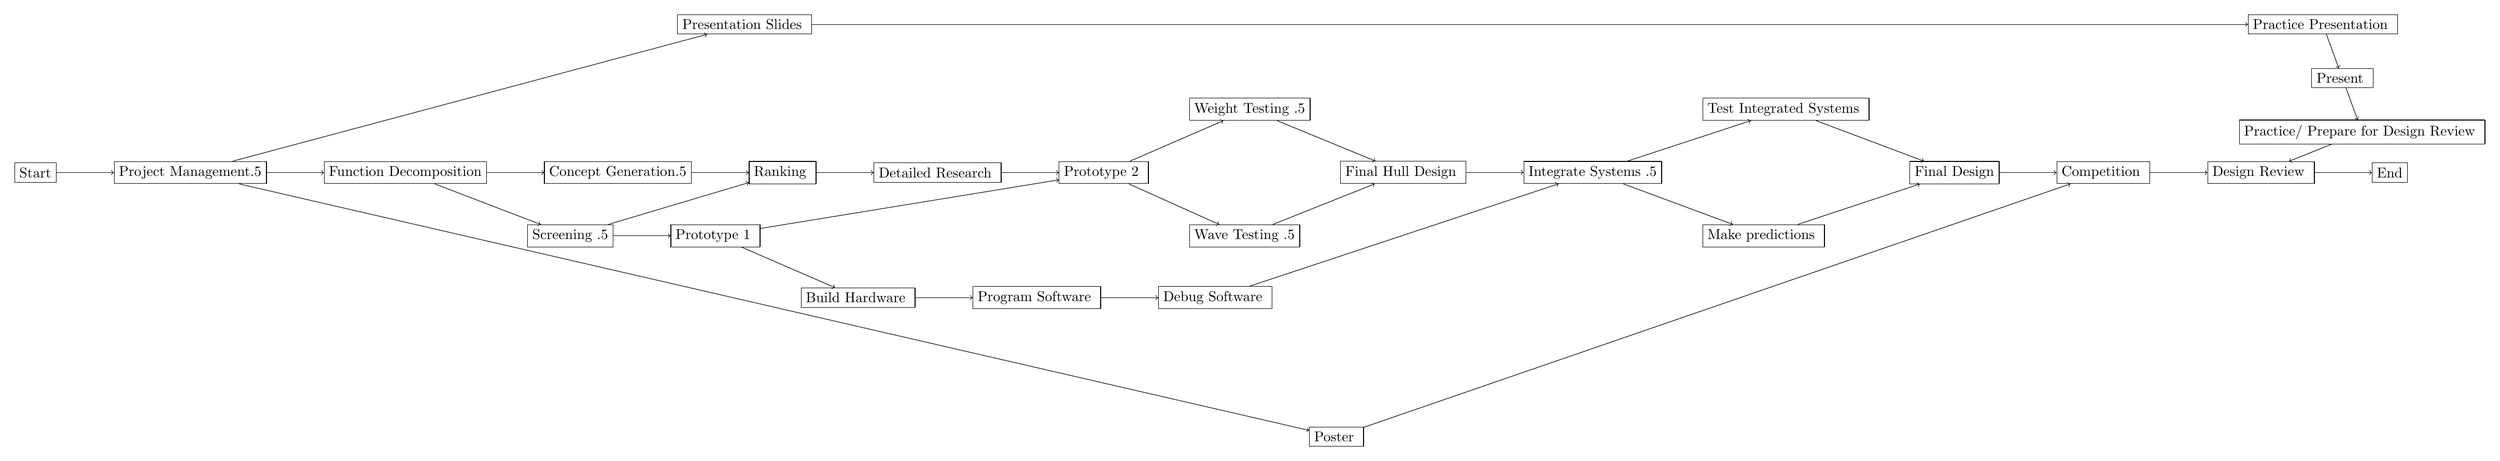
\begin{tikzpicture}[
	node distance=4em,
	every on chain/.style={
		join,
		rectangle split,
		rectangle split horizontal,
		rectangle split parts=2,
		rectangle split ignore empty parts,
		align=center,
		draw,
	},
	every join/.style={->},
]
{
	[start chain=main]
	\node (start) [on chain] {Start};

	\node (projectmanagement) [on chain] {\task Project Management\time 0.5};

	{ [start branch]
		\node (slides) [on chain=going {at=(\tikzchainprevious), shift=(15:20em)}] {\task Presentation Slides \time 2};
		\node (practice) [on chain=going {at=(\tikzchainprevious), shift=(0:55em)}] {\task Practice Presentation \time 1};
		\node (present) [on chain=going {at=(\tikzchainprevious), shift=(-70:2em)}] {\task Present \time 1};
		\node (prepdesignreview) [on chain=going {at=(\tikzchainprevious), shift=(-70:2em)}] {\task Practice/ Prepare for Design Review \time 2};
	}

	{ [start branch]
		\node (poster) [on chain=going {at=(\tikzchainprevious), shift=(-13:41em)}] {\task Poster \time 3};
	}

	\node (functiondecomp) [on chain] {\task Function Decomposition\time1};

	{ [start branch=screen]
		\node (screening) [on chain=going below right] {\task Screening \time0.5};
		\node (prototype1) [on chain] {\task Prototype 1 \time1};
		\node (buildhw) [on chain=going below right] {\task Build Hardware \time 2};
		\node (program) [on chain] {\task Program Software \time 2};
		\node (debug) [on chain] {\task Debug Software \time 1};
	}

	\node (conceptgeneration) [on chain] {Concept Generation\time1.5};
	\node (ranking) [on chain, join=with screening] {\task Ranking \time1};

	\node (research) [on chain] {\task Detailed Research \time2};
	\node (prototype2) [on chain, join=with prototype1] {\task Prototype 2 \time 2};
	{ [start branch]
		\node (weighttest) [on chain=going above right] {\task Weight Testing \time 0.5};
	}
	\node (wavetest) [on chain=going below right] {\task Wave Testing \time 0.5};

	\node (hulldesign) [on chain=going above right, join=with weighttest] {\task Final Hull Design \time 1};

	\node (integrate) [on chain, join=with debug] {\task Integrate Systems \time 0.5};

	{ [start branch]
		\node (predict) [on chain=going below right] {\task Make predictions \time 2};
	}

	\node (testint) [on chain=going above right] {\task Test Integrated Systems \time 2};

	\node (final) [on chain=going below right, join=with predict] {Final Design};

	\node (competition) [on chain, join=with poster] {\task Competition \time 1};

	\node (designreview) [on chain, join=with prepdesignreview] {\task Design Review \time 1};

	\node (end) [on chain] {End};

%	{ [start branch=prototype]
%		\node (prototypetesting) [on chain=going {at=(\tikzchainprevious), shift=(-15:15em)}] {Prototype Testing\time3};
%	}
%	\node [on chain] {Ranking\time1};
%	\node (scoring) [on chain] {Scoring\time2};
%	{ [start branch=design]
%		\node [on chain=going above right] {Design in Detail\time9};
%	}
%	{ [start branch=ordering]
%		\node [on chain=going below right] {Ordering\time6};
%	}
%	\node (building) [on chain] {Building\time10};
%	\node (competition) [
%		on chain,
%		join=with main/design-end,
%		join=with main/ordering-end,
%		join=with main/poster-end,
%		join=with main/prototype-end,
%	] {Competition\time1};
%	{ [continue branch=report]
%		\node (conclusion) [on chain=going {at=(\tikzchainprevious), shift=(0:37em)},join=with competition] {\nodepart[text width=8em]{one} Conclusion and Recommendation\time2};
%		%\node (editconclusion) [on chain=going {at=(\tikzchainprevious),shift=(-55:1.5)}] {Edit Conclusion\time2};
%		\node (editconclusion) [on chain, right=of competition] {Edit Conclusion\time2};
%		\node (end) [
%			on chain,
%			join=with main/presentation-end,
%			join=with main/report/editbody-end,
%		] {End};
%	}
}
\end{tikzpicture}

\end{document}

